
\documentclass[sigconf,authordraft]{acmart}

\AtBeginDocument{%
  \providecommand\BibTeX{{%
    Bib\TeX}}}

\setcopyright{acmlicensed}
\copyrightyear{2024}
\acmYear{2024}
\acmDOI{XXXXXXX.XXXXXXX}

\acmConference[TEI '25]{19th International Conference on Tangible Embedded and Embodied Interaction}{March 04--07,
  2025}{Bordeaux, France}
\acmISBN{978-1-4503-XXXX-X/18/06}


\begin{document}

%%
%% The "title" command has an optional parameter,
%% allowing the author to define a "short title" to be used in page headers.
\title{RadioResonance: A Tangible Interface to Explore Archived Sound of Warfare}

%%
%% The "author" command and its associated commands are used to define
%% the authors and their affiliations.
%% Of note is the shared affiliation of the first two authors, and the
%% "authornote" and "authornotemark" commands
%% used to denote shared contribution to the research.
\author{Kosuke Shimizu}
\email{shimizu@ai.iit.tsukuba.ac.jp}
\orcid{0009-0007-5689-1331}
\affiliation{%
  \institution{University of Tsukuba}
  \city{Tsukuba}
  \state{Ibaraki}
  \country{Japan}
}
\author{Kenji Suzuki}
\email{kenji@ieee.org}
\affiliation{%
  \institution{University of Tsukuba}
  \city{Tsukuba}
  \state{Ibaraki}
  \country{Japan}
}

%%
%% By default, the full list of authors will be used in the page
%% headers. Often, this list is too long, and will overlap
%% other information printed in the page headers. This command allows
%% the author to define a more concise list
%% of authors' names for this purpose.
\renewcommand{\shortauthors}{Shimizu}

%%
%% The abstract is a short summary of the work to be presented in the
%% article.
\begin{abstract}
RadioResonance is an interactive art installation that reimagines the exploration of historical audio archives through a tangible radio interface. The installation consists of a modified vintage radio that serves as a tangible interface to navigate through time, geography, and content types of World War II era broadcasts. Users interact with familiar radio controls - tuning dials, antenna positioning, and effect switches - to access and compare different aspects of the wartime soundscape. The frequency dial navigates the timeline, the antenna directs geographical focus, and switches alter content types between news, propaganda, and civilian accounts. By emphasizing audio over visual content, the system reduces cognitive load and allows for more intuitive processing of historical information. Our goal is to make the exploration of complex historical narratives more accessible and engaging, particularly for younger generations.
\end{abstract}

%%
%% The code below is generated by the tool at http://dl.acm.org/ccs.cfm.
%% Please copy and paste the code instead of the example below.
%%
\begin{CCSXML}
<ccs2012>
 <concept>
  <concept_id>10003120.10003121.10003122.10003123</concept_id>
  <concept_desc>Human-centered computing~Interactive systems and tools</concept_desc>
  <concept_significance>500</concept_significance>
 </concept>
 <concept>
  <concept_id>10003120.10003121.10003129</concept_id>
  <concept_desc>Human-centered computing~Interaction devices</concept_desc>
  <concept_significance>300</concept_significance>
 </concept>
 <concept>
  <concept_id>10002944.10011122.10011134</concept_id>
  <concept_desc>Applied computing~Interactive learning environments</concept_desc>
  <concept_significance>200</concept_significance>
 </concept>
 <concept>
  <concept_id>10003120.10003123.10003130</concept_id>
  <concept_desc>Human-centered computing~Sound-based input / output</concept_desc>
  <concept_significance>100</concept_significance>
 </concept>
</ccs2012>
\end{CCSXML}

\ccsdesc[500]{Human-centered computing~Interactive systems and tools}
\ccsdesc[300]{Human-centered computing~Interaction devices}
\ccsdesc[200]{Applied computing~Interactive learning environments}
\ccsdesc[100]{Human-centered computing~Sound-based input / output}


%%
%% Keywords. The author(s) should pick words that accurately describe
%% the work being presented. Separate the keywords with commas.
\keywords{Tangible Interface, Digital Archive Representation, Search Engine}
%% A "teaser" image appears between the author and affiliation
%% information and the body of the document, and typically spans the
%% page.
\begin{teaserfigure}
  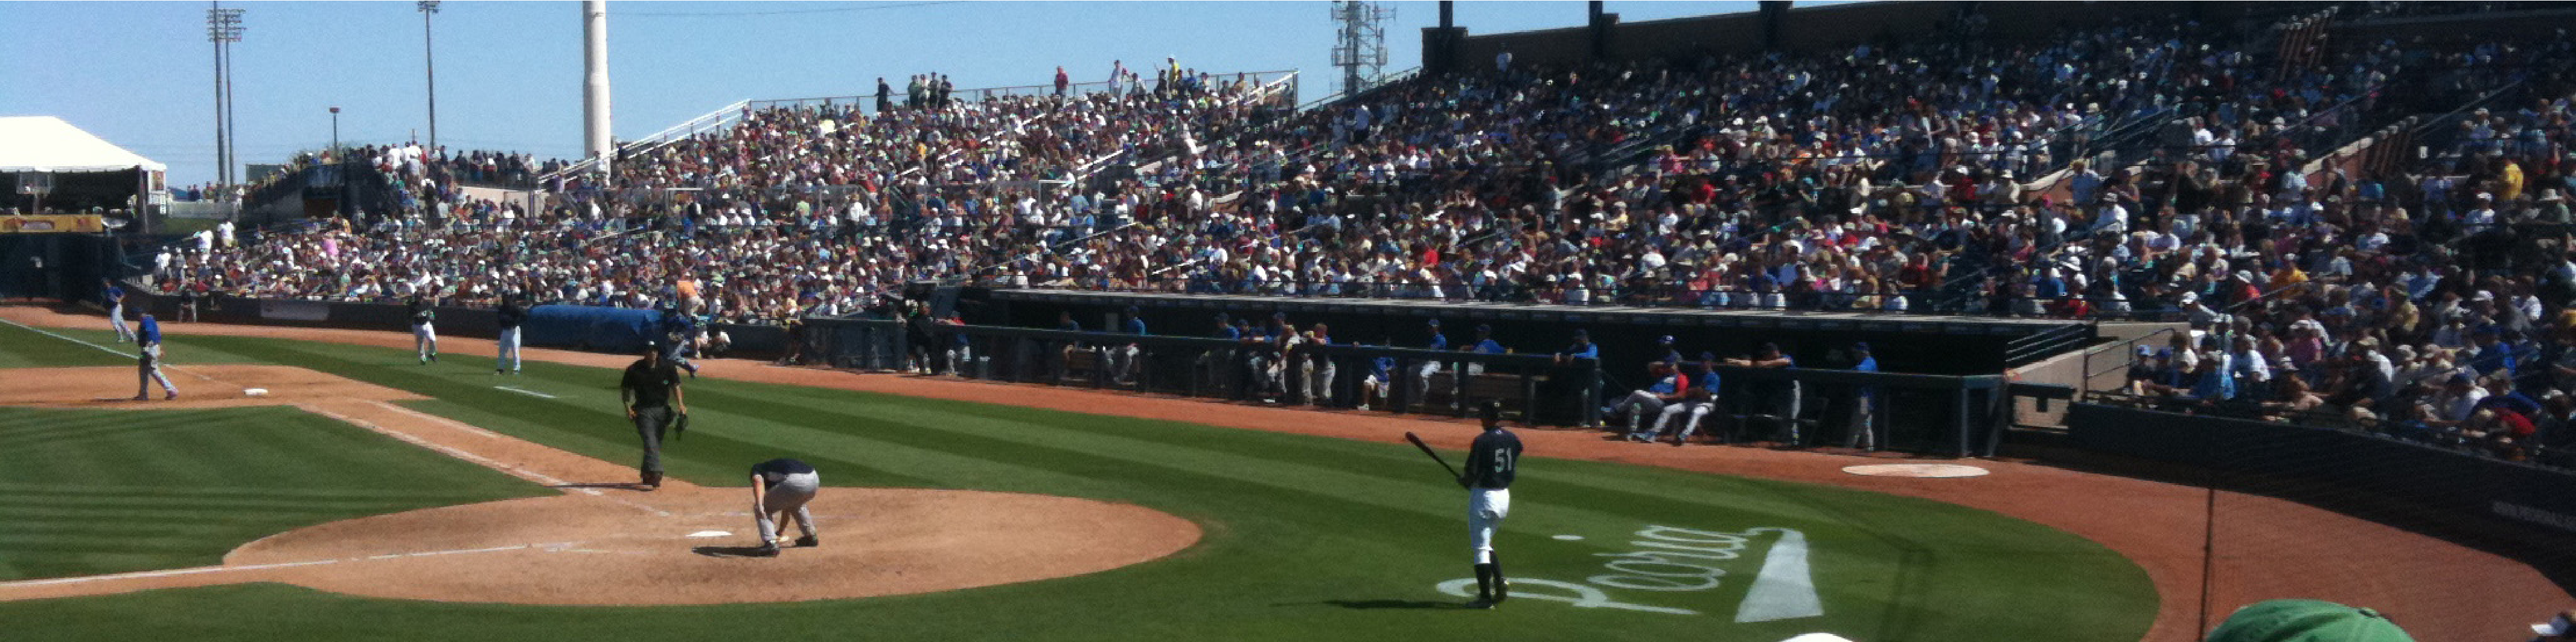
\includegraphics[width=\textwidth]{sampleteaser}
  \caption{Seattle Mariners at Spring Training, 2010.}
  \Description{Enjoying the baseball game from the third-base
  seats. Ichiro Suzuki preparing to bat.}
  \label{fig:teaser}
\end{teaserfigure}

\received{20 February 2007}
\received[revised]{12 March 2009}
\received[accepted]{5 June 2009}

%%
%% This command processes the author and affiliation and title
%% information and builds the first part of the formatted document.
\maketitle

\section{Introduction}


\section{Method}
The system is designed with three components. As a body of system, we employed old discard radio with two dial and anthena. Raspberry pi 5 is employed as a main computational system, and Raspberry Pi Camera Module 3 Wide is used as a computer vision. 
\subsection{ReDesingning location input}
In order to precisely incorporate user's location input, we attached LED light on antenna and developed a system to convert lighted area to positional information. The system first detect lighted area from computer vision, second calculate the actual area from image source with homography matrix conversion. We adopt equidistant cylindrical projection method for printed maps so that we can easily transform between pixel coordinates and geographic coordinates, which enables straightforward perspective correction and seamless integration with computer vision libraries.
The conversion from image coordinates $(u,v)$ to geographic coordinates $(\phi,\lambda)$ can be expressed as:
\begin{equation}
\begin{bmatrix} u' \\ v' \\ 1 \end{bmatrix} = 
H \begin{bmatrix} u \\ v \\ 1 \end{bmatrix}
\end{equation}
where $H$ is the homography matrix that corrects for perspective distortion. The corrected coordinates $(u',v')$ are then transformed to geographic coordinates using:
\begin{equation}
\lambda = \frac{u'}{W} \cdot 360° - 180°
\end{equation}
\begin{equation}
\phi = 90° - \frac{v'}{H} \cdot 180°
\end{equation}
where $W$ and $H$ are the width and height of the reference map in pixels. This linear transformation is particularly efficient as it requires minimal computational overhead while maintaining sufficient accuracy for practical applications. The system achieves an average positional error of $\pm x$ meters in our experimental validation, demonstrating its viability for location-based applications.

\subsection{Input of audio type and time}



\section{Research Statement}
This sysytem contributes to the field of historical education through the application of Tangible User Interfaces (TUI). Building on the foundational work of Ishii \verb|&| Ullmer, our system leverages physical interactions to navigate complex historical narratives\cite{tangible}. The radio metaphor serves as an intuitive interface, allowing users to explore temporal and spatial dimensions of war history through familiar tactile interactions. The effectiveness of this approach is supported by Petrelli et al.\cite{Petrelli}, who argue that tangible interactions with historical content can foster deeper personal engagement and reflection. 
Our multimodal presentation strategy, combining auditory and supplementary visual information, is informed by Moreno verb\verb|&| Mayer's cognitive theory of learning\cite{Moreno} and Boltz\cite{boltz}identifies sound is a powerful contextual cues for memory and emotional response.
The design aligns with Shneiderman's\cite{Mantra} information visualization mantra, "Overview first, zoom and filter, then details-on-demand," enabling users to process and discover patterns in large volumes of historical data effectively. This approach is further grounded in exploratory learning principles\cite{bruner}, encouraging active exploration and comparison of information across different time periods and regions.

\section{Artistic Statement}
In the past, radio was the interface between the battlefield and the home front, bringing distant echoes of conflict into living rooms across the world. Today, we re-imagine this once-ubiquitous device as a bridge spanning not space, but time. Our system transforms the radio into an interface between those who have known war and those who have not, between memory and imagination, between history and the present.
Our work builds upon previous efforts to make historical archives more accessible and engaging. Projects like the United States Holocaust Memorial Museum's oral history archive and the Imperial War Museums' sound collection have demonstrated the power of audio in preserving and sharing wartime experiences. We extend this approach by introducing an interactive, tangible element that encourages active exploration.

Central to our design is the concept of playful learning. By invoking curiosity through tangible interaction, we invite users to discover war history as a multifaceted narrative. The act of tuning the radio, adjusting antennas, and switching between channels becomes a journey of discovery. Users encounter snippets of information that spark interest, prompting them to delve deeper into original documentation within digital archives.
While digital archiving initiatives have proliferated, methods for effectively utilizing these vast resources remain underdeveloped. Our project addresses this gap by proposing a novel approach to archive engagement. We argue that the value of digital archives extends beyond mere preservation; it lies in their potential to foster new forms of interaction with historical material.

This installation thus serves a dual purpose: it offers an immersive, emotive experience of war history while simultaneously acting as a gateway to more comprehensive archival resources. By blending the familiar tactility of radio operation with the depth of digital archives, we aim to create a bridge between casual curiosity and scholarly inquiry, making the exploration of war history both accessible and profound.

\section{Limitation and Future work}
We have developed artistic installation, aiming to design digital archive of WW2 with tangible interface. Participant can easily explore archived. 


\section{Acknowledgments}


\bibliographystyle{ACM-Reference-Format}
\bibliography{citation}

\end{document}
